\section{Casi d'uso}

\subsection{Attori dei casi d'uso}

\subsubsection{Attori primari}
\begin{figure}[H]
		\centering
		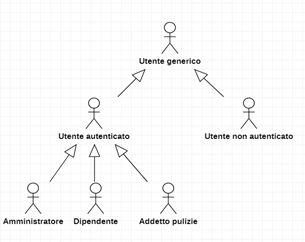
\includegraphics[width=10cm]{res/images/utentigenerali.png}
		\caption{Gerarchia degli attori principali}
		\label{fig:Gerarchia attori principali}
	\end{figure}

\textbf{Utente generico}\\
Si riferisce a un utente generico che accede alla piattaforma.\\
\\
\textbf{Utente non autenticato}\\
Si riferisce a un utente generico che non ha ancora effettuato l’autenticazione alla piattaforma.\\
\\
\textbf{Utente autenticato}\\
Si riferisce a un utente generico che si è autenticato nel sistema con la procedura di login.\\
\\
\textbf{Amministratore}\\
Si riferisce a un utente che si è autenticato nel sistema con il ruolo di amministratore.\\
\\
\textbf{Dipendente}\\
Si riferisce a un utente che si è autenticato nel sistema con il ruolo di dipendente.\\
\\
\textbf{Addetto pulizie}\\
Si riferisce a un utente che si è autenticato nel sistema con il ruolo di addetto alle pulizie.\\

\subsubsection{Attori secondari}
\textbf{Tag RFID}\\
Si riferisce ai tag presenti sulle postazioni. Ogni tag è assegnato a una postazione e permette di identificarla digitalmente.\\
\\
\textbf{Ethereum}\\
Si riferisce al servizio che memorizza su blockchain gli eventi di occupazione e igienizzazione delle postazioni.\\

\subsection{Elenco dei casi d'uso}
In questa sezione sono riportati tutti i casi d'uso individuati, ordinati per attore principale. Quando ritenuto utile, essi sono accompagnati da un grafico.
\\
\subsubsection{ UC1 - Guida introduttiva}
\begin{itemize}
           	\item\textbf{Attori Primari:} utente generico.
           	\item\textbf{Descrizione:} l'utente riceve una guida riguardo il login e il funzionamento.
           	\item\textbf{Scenario principale:} l’utente accede alla pagina introduttiva e visualizza la guida.
           	\item\textbf{Precondizione:} il sistema è raggiungibile e funzionante, l’utente accede alla pagina iniziale del sito della piattaforma.
           	\item\textbf{Postcondizione:} il sistema fornisce all’utente, attraverso la lettura della guida, tutte le istruzioni necessarie a effettuare il login.
\end{itemize}

\subsubsection{ UC2 - Login}
\begin{itemize}
           	\item\textbf{Attori Primari:} utente non autenticato.
           	\item\textbf{Descrizione:} l’utente tenta di autenticarsi all'applicativo.
           	\item\textbf{Scenario principale:} l’utente non è ancora autenticato ed esegue il login.
           	\item\textbf{Precondizione:} l’utente non si è autenticato nell'applicativo. 
           	\item\textbf{Postcondizione:} l’utente si è autenticato con successo, ed è stato identificato dal sistema
           	nel ruolo di amministratore, dipendente o addetto alle pulizie. A seconda della tipologia di utente vengono rese
           	disponibili diverse funzionalità.
\end{itemize}

\subsubsection{ UC2.1 - Visualizzazione messaggio di errore}
\begin{itemize}
	\item\textbf{Attori Primari:} utente non autenticato.
	\item\textbf{Descrizione:} l'utente visualizza un messaggio di errore dovuto al fatto che ha tentato il login ma ha sbagliato a inserire le credenziali.
	\item\textbf{Scenario principale:} l’utente tenta di eseguire la procedura di login all'applicativo.
	\item\textbf{Precondizione:} l'utente tenta di autenticarsi nell'applicativo.
	\item\textbf{Postcondizione:} viene visualizzato un messaggio di errore per informare l'utente del fatto che ha sbagliato a inserire le credenziali.
\end{itemize}
\subsubsection{ UC2.2 - Visualizzazione schermata relativa a utente non abilitato}
\begin{itemize}
           	\item\textbf{Attori Primari:} utente non autenticato.
           	\item\textbf{Descrizione:} l'utente tenta di autenticarsi nell'applicativo, tuttavia a causa della disabilitazione del suo account, il login viene interrotto, e
           	l'utente visualizza il messaggio di errore che illustra la causa della disabilitazione dell'account.
           	\item\textbf{Scenario principale:} l’utente non autenticato con account disabilitato tenta di autenticarsi. 
           	La procedura di autenticazione viene bloccata a causa dello stato dell'account.
           	\item\textbf{Precondizione:} un utente non autenticato, registrato all'applicativo e con account disabilitato tenta di effettuare il login automatico. 
           	\item\textbf{Postcondizione:} viene visualizzato un messaggio di errore per informare l'utente del fatto che il 
           	proprio account è stato disabilitato dall'amministratore. Se quest'ultimo, durante la procedura di disabilitazione, ha inserito un messaggio contenente la causa di tale azione, allora tale messaggio viene visualizzato.
\end{itemize}

\subsubsection{ UC3 - Logout}
\begin{itemize}
	\item\textbf{Attori Primari:} 
	utente autenticato.
	\item\textbf{Descrizione:} 
	l'utente si disautentica dal sistema.
	\item\textbf{Scenario principale:} 
	l'utente autenticato preme un pulsante per la disautenticazione ed essa viene eseguita.
	\item\textbf{Precondizione:} 
	l'utente è autenticato nel sistema.
	\item\textbf{Postcondizione:}
	l'utente non è autenticato nel sistema.
\end{itemize}


\subsubsection{ UC4 - Gestione stanze e postazioni}
\begin{figure}[H]
	\centering
	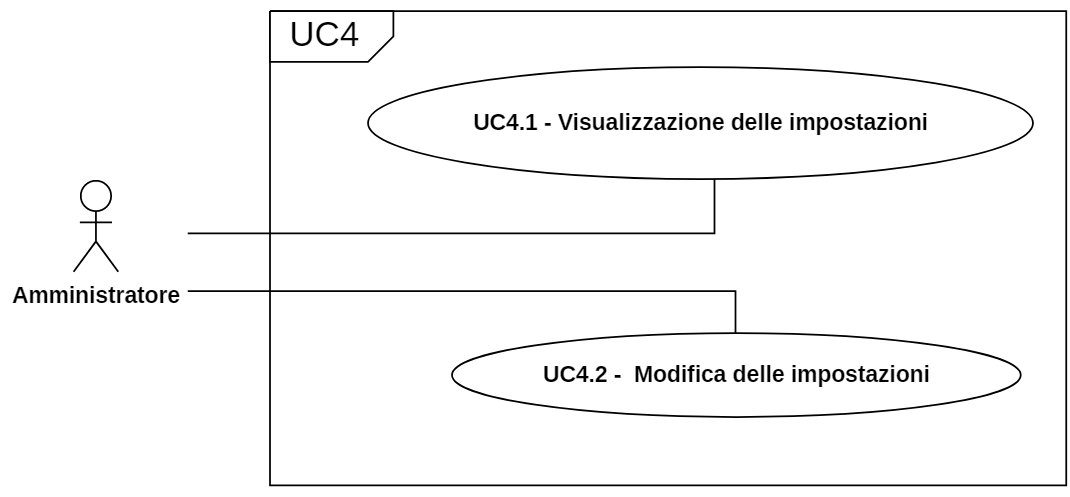
\includegraphics[width=18cm]{res/images/UC4.png}
	\caption{Gestione stanze e postazioni}
	\label{fig:Gestione stanze e postazioni}
\end{figure}
\begin{itemize}
           	\item\textbf{Attori Primari:} 
           	amministratore.
           	\item\textbf{Descrizione:} 
           	l'amministratore visualizza, crea e modifica le caratteristiche di stanze e postazioni al loro interno.
           	\item\textbf{Scenario principale:} 
           	l'amministratore raggiunge l'area di gestione delle stanze e delle postazioni. Da lì può eseguire le azioni di visualizzazione, creazione e modifica.
           	\item\textbf{Precondizione:} 
           	l'utente è autenticato come amministratore.
           	\item\textbf{Postcondizione:}
           	l'utente ha eseguito delle azioni di gestione delle stanze o delle postazioni.
\end{itemize}

\subsubsection{ UC4.1 - Visualizzazione stanze e postazioni}
\begin{itemize}
	\item\textbf{Attori Primari:}
	amministratore.
	\item\textbf{Descrizione:}
	il sistema mostra all'amministratore lo schema delle stanze e delle postazioni aggiornato rispetto alle azioni salvate su Ethereum.
	\item\textbf{Scenario principale:}
	l'amministratore raggiunge la pagina di visione delle stanze delle postazioni e le visualizza. Le postazioni sono colorate in base al loro stato e gli stati possibili sono:
	\begin{itemize}
		\item[$-$] libera e igienizzata;
		\item[$-$] libera e non igienizzata;
		\item[$-$] occupata;
		\item[$-$] prenotata e igienizzata;
		\item[$-$] prenotata e non igienizzata;
		\item[$-$] inaccessibile.
	\end{itemize}
	per ogni stanza è indicato il numero di occupanti attuali.
	\item\textbf{Estensioni:}
	visualizzazione a calendario delle postazioni prenotate (UC4.1.1)
	\item\textbf{Precondizione:} 
	l'utente è autenticato come amministratore.
	\item\textbf{Postcondizione:}
	l'amministratore visualizza lo schema delle stanze e delle postazioni.
\end{itemize}

\subsubsection{ UC4.1.1 - Visualizzazione a calendario delle postazioni prenotate}
\begin{itemize}
	\item\textbf{Attori Primari:}
	amministratore.
	\item\textbf{Descrizione:}
	il sistema mostra all'amministratore un calendario con le prenotazioni delle postazioni.
	\item\textbf{Scenario principale:}
	l'utente raggiunge l'area di visualizzazione del calendario delle prenotazioni delle postazioni e lo visualizza.
	\item\textbf{Precondizione:} 
	l'utente è autenticato come amministratore.
	\item\textbf{Postcondizione:}
	l'amministratore visualizza il calendario delle prenotazioni delle postazioni.
\end{itemize}

\subsubsection{ UC4.2 - Creazione di una stanza}
\begin{itemize}
	\item\textbf{Attori Primari:}
	amministratore.
	\item\textbf{Attori Secondari:}
	Ethereum.
	\item\textbf{Descrizione:} 
	l'utente aggiunge una stanza al sistema.
	\item\textbf{Scenario principale:} 
	l'utente autenticato preme un pulsante per creare una nuova stanza. Compare quindi il campo "Nome della stanza" da compilare.
	L'utente compila il campo e preme un pulsante per confermare la creazione della stanza.
	Se non è gia presente una stanza con il codice inserito, essa viene creata e la sua configurazione viene inviata a Ethereum per essere salvata.
	\item\textbf{Estensione:}
	se è gia presente una stanza con lo stesso nome l'utente viene avvisato (UC4.2.1).
	\item\textbf{Precondizione:} 
	l'utente è autenticato come amministratore.
	\item\textbf{Postcondizione:}
	è stata aggiunta una stanza vuota con le caratteristiche specificate.
\end{itemize}

\subsubsection{ UC4.2.1 - Avviso nome stanza già utilizzato}
\begin{itemize}
	\item\textbf{Attori Primari:}
	amministratore.
	\item\textbf{Descrizione:}
	l'utente tenta di assegnare alla stanza che sta creando un nome già utilizzato per un'altra stanza nel sistema e ne viene avvisato.
	\item\textbf{Scenario principale:}
	l'utente sta creando una stanza e inserisce come nome un valore già utilizzato.
	La stanza non viene creata e alla vista dell'utente compare un avviso che indica che il nome è già stato utilizzato.
	\item\textbf{Precondizione:}
	l'utente si trova sulla pagina di creazione di una stanza.
	\item\textbf{Postcondizione:}
	l'utente visualizza il messaggio d'errore.
\end{itemize}

\subsubsection{ UC4.3 - Eliminazione di una stanza}
\begin{itemize}
	\item\textbf{Attori Primari:}
	amministratore.
	\item\textbf{Attori Secondari:}
	Ethereum.
	\item\textbf{Descrizione:} 
	l'utente elimina dal sistema una stanza con tutte le postazioni in essa presenti.
	\item\textbf{Scenario principale:} 
	l'utente preme sul pulsante per l'eliminazione di una stanza. La stanza viene eliminata dal sistema con tutte le postazioni al suo interno e l'azione viene comunicata a Ethereum.
	\item\textbf{Precondizione:} 
	l'utente è autenticato.
	\item\textbf{Postcondizione:}
	è stata eliminata la stanza specificata, con tutte le postazioni al suo interno.
\end{itemize}

\subsubsection{UC4.4 - Modifica di una stanza}
\begin{itemize}
	\item\textbf{Attori Primari:}
	amministratore.
	\item\textbf{Descrizione:}
	l'utente modifica il codice identificativo di una stanza.
	\item\textbf{Scenario principale:} 
	l'utente preme un pulsante per la modifica di una stanza. Gli viene chiesto di inserire il nuovo nome e di confermare la modifica. La stanza ha ora il nome aggiornato.
	\item\textbf{Estensioni:}
	\begin{itemize}
		\item[$-$] rendere una stanza inaccessibile per alcuni giorni (UC4.4.1);
		\item[$-$] se è già presente una stanza con lo stesso nome l'utente viene avvisato (UC4.2.1).
	\end{itemize}
	\item\textbf{Precondizione:} 
	l'utente è autenticato.
	\item\textbf{Postcondizione:}
	il codice della stanza selezionata è stato modificato.
\end{itemize}

\subsubsection{UC4.4.1 - Impostazione di una stanza come inaccessibile.}
\begin{itemize}
	\item\textbf{Attori Primari:}
	amministratore.
	\item\textbf{Descrizione:}
	l'utente rende una stanza inaccessibile per alcuni giorni.
	\item\textbf{Scenario principale:} 
	l'utente imposta le date di inizio e fine del periodo di inaccessibilità della stanza e conferma l'impostazione attraverso un pulsante.
	\item\textbf{Estensioni:}
	\begin{itemize}
		\item[$-$] cancellazione delle prenotazioni per quella postazione e notifica agli utenti che avevano prenotato (UC4.6.1).
	\end{itemize}
	\item\textbf{Precondizione:} 
	l'utente è autenticato come amministratore e ha raggiunto l'area dedicata a questa azione.
	\item\textbf{Postcondizione:}
	il codice della stanza selezionata è stato modificato.
\end{itemize}

\subsubsection{UC4.5 - Creazione di una postazione}
\begin{itemize}
	\item\textbf{Attori Primari:}
	amministratore.
	\item\textbf{Attori Secondari:}
	Ethereum.
	\item\textbf{Descrizione:}
	l'amministratore crea una postazione e la assegna a una stanza.
	\item\textbf{Scenario principale:} 
	l'amministratore preme un pulsante per aggiungere una nuova postazione. Gli viene chiesto di inserire i seguenti campi:
	\begin{itemize}
		\item[$-$] codice della postazione;
		\item[$-$] codice del tag RFID che identifica la postazione.
	\end{itemize}
	inoltre gli viene chiesto di indicare la posizione della postazione su una scacchiera rappresentante la stanza.
	L'amministratore preme un bottone per la conferma dei dati e la postazione viene aggiunta all'interno della stanza. La nuova configurazione della stanza viene comunicata a Ethereum.
	\item\textbf{Estensioni:}
	\begin{itemize}
		\item[$-$] avviso codice postazione già presente (UC4.5.1);
		\item[$-$] avviso codice tag già presente (UC4.5.2).
	\end{itemize}
	\item\textbf{Precondizione:} 
	l'utente è autenticato.
	\item\textbf{Postcondizione:}
	è stata inserita una nuova postazione all'interno di una stanza.
\end{itemize}



\subsubsection{UC4.5.1 - Avviso codice postazione già utilizzato}
\begin{itemize}
	\item\textbf{Attori Primari:}
	amministratore.
	\item\textbf{Descrizione:}
	l'utente tenta di assegnare a una postazione un codice già utilizzato attualmente per un'altra.
	\item\textbf{Scenario principale:}
	l'utente sta creando o modificando una postazione e inserisce come codice un valore già utilizzato.
	La postazione non viene creata e alla vista dell'utente compare un avviso che indica che il codice è attualmente utilizzato.
	\item\textbf{Precondizione:}
	l'utente si trova sulla pagina di creazione o quella di modifica di una postazione.
	\item\textbf{Postcondizione:}
	l'utente visualizza il messaggio d'errore.
\end{itemize}

\subsubsection{UC4.5.2 - Avviso codice tag già utilizzato}
\begin{itemize}
	\item\textbf{Attori Primari:}
	amministratore.
	\item\textbf{Descrizione:}
	l'utente tenta di assegnare a una postazione il codice di un tag già utilizzato attualmente per un'altra.
	\item\textbf{Scenario principale:}
	l'utente sta creando o modificando una postazione e inserisce come codice del tag corrispondente un valore già utilizzato.
	La postazione non viene creata e alla vista dell'utente compare un avviso che indica che il codice del tag è già assegnato a una postazione.
	\item\textbf{Precondizione:}
	l'utente si trova sulla pagina di creazione o quella di modifica di una postazione.
	\item\textbf{Postcondizione:}
	l'utente visualizza il messaggio d'errore.
\end{itemize}

\subsubsection{UC4.6 - Eliminazione di una postazione}
\begin{itemize}
	\item\textbf{Attori Primari:}
	amministratore.
	\item\textbf{Attori Secondari:}
	Ethereum.
	\item\textbf{Descrizione:}
	l'utente elimina una postazione.
	\item\textbf{Scenario principale:} 
	l'utente raggiunge l'area di eliminazione delle postazioni, ne seleziona una ed esegue l'eliminazione. La nuova configurazione della stanza viene inviata a Ethereum.
	\item\textbf{Estensioni:}
	\begin{itemize}
		\item[$-$] cancellazione delle prenotazioni per quella postazione e notifica agli utenti che avevano prenotato (UC4.6.1).
	\end{itemize}
	\item\textbf{Precondizione:} 
	l'utente è autenticato come amministratore.
	\item\textbf{Postcondizione:}
	una postazione è stata eliminata.
\end{itemize}

\subsubsection{ UC4.6.1 - Avviso agli utenti che hanno prenotato}
\begin{itemize}
	\item\textbf{Attori Primari:}
	amministratore.
	\item\textbf{Attori Secondari:}
	dipendente.
	\item\textbf{Descrizione:}
	gli utenti che hanno prenotato una postazione che non è più disponibile vengono avvisati.
	\item\textbf{Scenario principale:}
	se l'amministratore esegue la modifica o l'eliminazione di una postazione i dipendenti vengono avvisati che le loro prenotazioni non sono più valide.
	\item\textbf{Precondizione:}
	l'utente è autenticato come amministratore e alcuni dipendenti hanno prenotato la postazione che verrà resa non disponibile.
	\item\textbf{Postcondizione:}
	la postazione non è disponibile e i dipendenti interessati sono stati avvisati.
\end{itemize}

\subsubsection{ UC4.7 - Modifica di una postazione}
\begin{itemize}
	\item\textbf{Attori Primari:}
	amministratore.
	\item\textbf{Attori Secondari:}
	Ethereum.
	\item\textbf{Descrizione:}
	l'utente modifica gli attributi di una postazione.
	\item\textbf{Scenario principale:} 
	l'utente preme sul pulsante per la modifica di una postazione. Gli vengono richiesti i nuovi dati da inserire e la nuova posizione della postazione. Il sistema invia i nuovi dati a Ethereum.
	\item\textbf{Estensioni:}
	\begin{itemize}
		\item[$-$] avviso codice postazione già presente (UC4.5.1);
		\item[$-$] avviso codice tag già presente (UC4.5.2).
	\end{itemize}
	\item\textbf{Precondizione:} 
	l'utente è autenticato come amministratore.
	\item\textbf{Postcondizione:}
	sono stati aggiornati gli attributi della postazione selezionata.
\end{itemize}

\subsubsection{ UC5 - Gestione credenziali}
\begin{figure}[H]
	\centering
	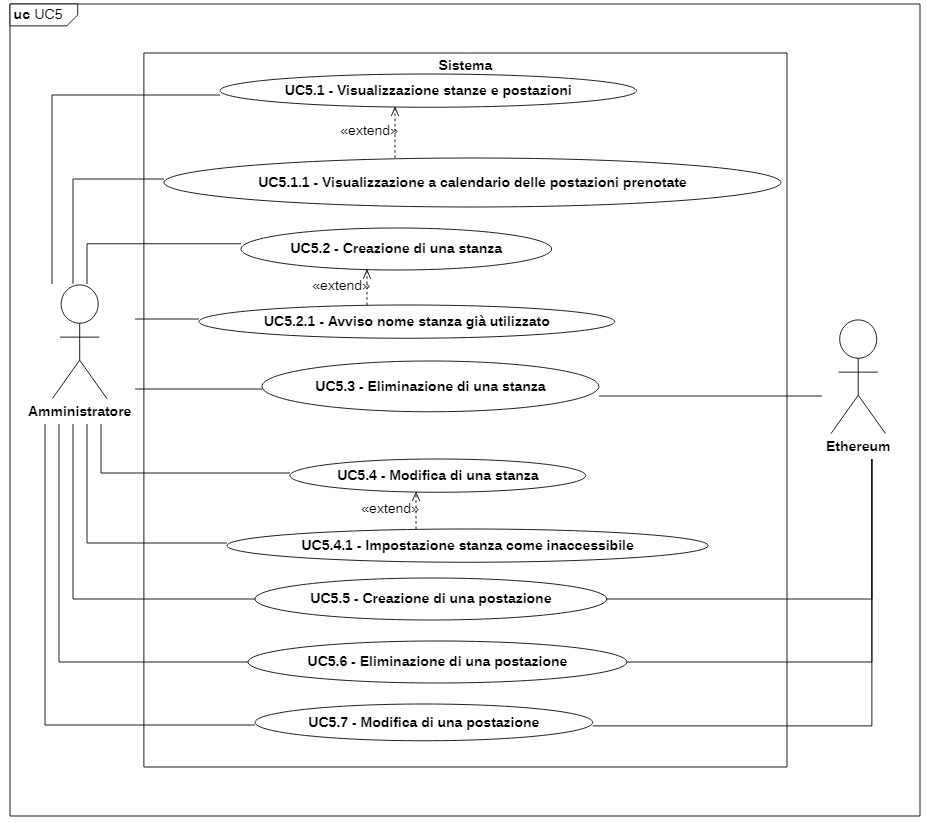
\includegraphics[width=15cm]{res/images/UC5.png}
	\caption{Gestione credenziali}
	\label{fig:Gestione credenziali}
\end{figure}
\begin{itemize}
           	\item\textbf{Attori Primari:}
           	amministratore.
           	\item\textbf{Descrizione:} 
           	l'amministratore visualizza, crea, modifica ed elimina le credenziali di tutti gli altri utenti.
           	\item\textbf{Scenario principale:} 
           	l'amministratore raggiunge l'interfaccia di gestione delle credenziali e da lì può operare su di esse.
           	\item\textbf{Precondizione:} 
           	l'utente è autenticato come amministratore.
           	\item\textbf{Postcondizione:}
           	l'utente ha visualizzato, creato, modificato oppure eliminato credenziali.
\end{itemize}

\subsubsection{ UC5.1 - Visualizzazione lista credenziali}
\begin{itemize}
	\item\textbf{Attori Primari:} 
	amministratore.
	\item\textbf{Descrizione:} 
	l'amministratore visualizza le credenziali di tutti gli utenti del sistema.
	\item\textbf{Scenario principale:} 
	l'utente naviga nell'interfaccia in modo da ottenere la visualizzazione delle credenziali.
	\item\textbf{Precondizione:} 
	l'utente è autenticato come amministratore.
	\item\textbf{Postcondizione:}
	l'utente visualizza la lista delle credenziali.
\end{itemize}

\subsubsection{ UC5.2 - Creazione di una credenziale}
\begin{itemize}
	\item\textbf{Attori Primari:}
	amministratore.
	\item\textbf{Descrizione:} 
	l'amministratore crea una credenziale riservata a un qualsiasi utente del sistema: amministratore, dipendente o addetto alle pulizie.
	\item\textbf{Scenario principale:} 
	l'amministratore naviga nell'interfaccia del sito web in modo da raggiungere l'ambiente di creazione delle credenziali.
	Il sito presenta all'utente i seguenti campi da compilare:
	\begin{itemize}
		\item[$-$] nome;
		\item[$-$] cognome;
		\item[$-$] nome utente;
		\item[$-$] password;
		\item[$-$] e-mail.
	\end{itemize}
	successivamente l'utente preme il pulsante per la conferma dei dati e la nuova credenziale viene salvata nel sistema.
	\item\textbf{Precondizione:} 
	l'utente è autenticato come amministratore.
	\item\textbf{Postcondizione:}
	l'utente ha creato una nuova credenziale.
\end{itemize}

\subsubsection{ UC5.3 - Modifica di una credenziale}
\begin{itemize}
	\item\textbf{Attori Primari:} 
	amministratore.
	\item\textbf{Descrizione:} 
	l'utente modifica i valori di un profilo utente.
	\item\textbf{Scenario principale:} 
	l'amministratore naviga nell'interfaccia del sito web per accedere all'ambiente di modifica delle credenziali.
	Il sito presenta all'utente i seguenti campi da modificare:
	\begin{itemize}
		\item[$-$] nome;
		\item[$-$] cognome;
		\item[$-$] nome utente;
		\item[$-$] password;
		\item[$-$] e-mail.
	\end{itemize}
	successivamente l'utente preme il pulsante per la conferma dei dati e i dati già salvati nel sistema vengono aggiornati.
	\item\textbf{Precondizione:} 
	l'utente è autenticato come amministratore.
	\item\textbf{Postcondizione:}
	l'utente ha modificato un profilo utente.
\end{itemize}

\subsubsection{ UC5.4 - Eliminazione di una credenziale}
\begin{itemize}
	\item\textbf{Attori Primari:} 
	amministratore.
	\item\textbf{Descrizione:} 
	l'amministratore elimina delle credenziali dal sistema.
	\item\textbf{Scenario principale:} 
	l'amministratore naviga nel sito web per raggiungere l'ambiente di eliminazione delle credenziali.
	L'amministratore preme sul pulsante per l'eliminazione delle credenziali.
	Le credenziali selezionate sono eliminate dal sistema.
	\item\textbf{Precondizione:} 
	l'utente è autenticato come amministratore.
	\item\textbf{Postcondizione:}
	le credenziali selezionate non sono più presenti nel sistema.
\end{itemize}

\subsubsection{ UC6 - Esplorazione occupazioni delle postazioni}
\begin{figure}[H]
	\centering
	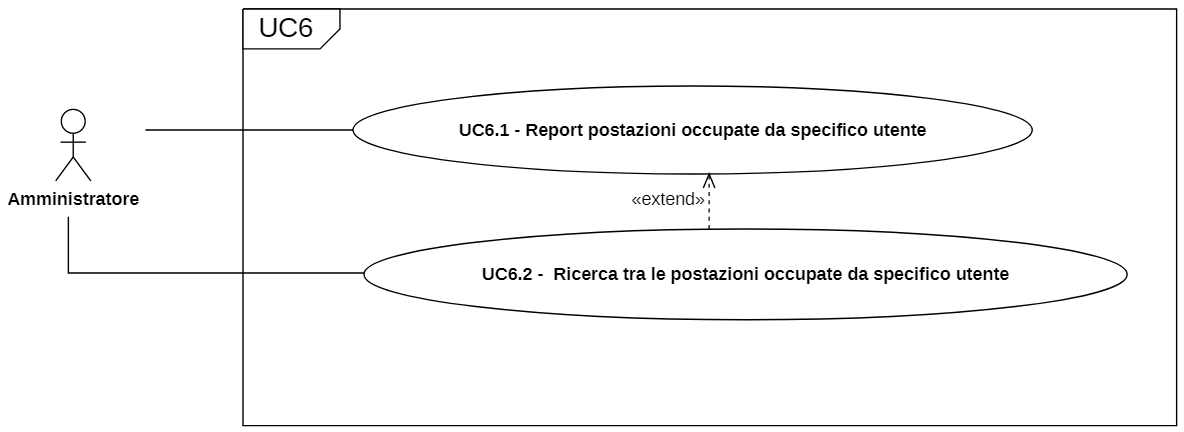
\includegraphics[width=18cm]{res/images/UC6.png}
	\caption{Esplorazione occupazioni delle postazioni}
	\label{fig:Esplorazione occupazioni delle postazioni}
\end{figure}
\begin{itemize}
	\item\textbf{Attori Primari:} 
	amministratore.
	\item\textbf{Descrizione:} 
	l'amministratore ottiene informazioni sugli eventi di occupazione.
	\item\textbf{Scenario principale:} 
	l'amministratore raggiunge la pagina per la ricerca delle occupazioni delle postazioni e ricerca le informazioni a cui è interessato.
	\item\textbf{Precondizione:} 
	l'utente è autenticato come amministratore.
	\item\textbf{Postcondizione:}
	l'utente visualizza le informazioni.
\end{itemize}

\subsubsection{ UC6.1 - Ottenimento report delle postazioni occupate da uno specifico utente}
\begin{itemize}
           	\item\textbf{Attori Primari:} 
           	amministratore.
           	\item\textbf{Descrizione:} 
           	l'amministratore ottiene informazioni in forma tabellare sulle postazioni occupate da uno specifico utente.
           	\item\textbf{Scenario principale:} 
           	l'amministratore raggiunge la pagina per la ricerca delle occupazioni delle postazioni e inserisce il nickname oppure il nome e cognome dell'utente a cui è interessato.
           	Nel report vengono visualizzate le date di inizio e fine delle occupazioni e i codici delle postazioni.
           	\item\textbf{Estensione:}
           	\begin{itemize}
           		\item[$-$] scaricamento del report delle occupazioni in un formato leggibile (UC6.3);
           		\item[$-$] ricerca tra le postazioni occupate da uno specifico utente (UC6.1.1).
           	\end{itemize}
           	\item\textbf{Precondizione:} 
           	l'utente è autenticato come amministratore.
           	\item\textbf{Postcondizione:}
           	l'utente visualizza le informazioni.
\end{itemize}

\subsubsection{ UC6.1.1 - Ricerca tra le postazioni occupate da uno specifico utente}
\begin{itemize}
	\item\textbf{Attori Primari:} 
	amministratore.
	\item\textbf{Descrizione:} 
	l'amministratore esegue una ricerca specifica tra le postazioni occupate.
	I valori che permettono di precisare la ricerca sono:
	\begin{itemize}
		\item[$-$] periodo all'interno del quale l'utente occupava la postazione.
	\end{itemize}
	\item\textbf{Scenario principale:} 
	l'amministratore seleziona i valori con cui vuole precisare la sua ricerca e ottiene la lista delle occupazioni con le relative informazioni.
	\item\textbf{Estensione:}
	\begin{itemize}
		\item[$-$] scaricamento del report delle occupazioni in un formato leggibile (UC6.3).
	\end{itemize}
	\item\textbf{Precondizione:} 
	l'utente si trova sulla pagina dedicata alla ricerca delle postazioni occupate.
	\item\textbf{Postcondizione:}
	l'utente visualizza le informazioni specificate dalla sua ricerca.
\end{itemize}

\subsubsection{ UC6.1.2 - Ottenimento report delle occupazioni di uno specifico utente con indicazione delle ore trascorse a ogni postazione}
\begin{itemize}
	\item\textbf{Attori Primari:} 
	amministratore.
	\item\textbf{Descrizione:} 
	l'amministratore ottiene informazioni in forma tabellare sulle postazioni occupate da uno specifico utente con l'indicazione delle ore trascorse in ogni postazione.
	\item\textbf{Scenario principale:} 
	l'amministratore raggiunge la pagina per la ricerca delle occupazioni delle postazioni e inserisce il nickname oppure il nome e cognome dell'utente a cui è interessato.
	Nel report vengono visualizzate le date di inizio e fine delle occupazioni, i codici delle postazioni e le ore trascorse.
	\item\textbf{Estensione:}
	\begin{itemize}
		\item[$-$] scaricamento del report delle occupazioni in un formato leggibile (UC6.3);
		\item[$-$] ricerca tra le postazioni occupate da uno specifico utente (UC6.1.1).
	\end{itemize}
	\item\textbf{Precondizione:} 
	l'utente è autenticato come amministratore.
	\item\textbf{Postcondizione:}
	l'utente visualizza le informazioni.
\end{itemize}

\subsubsection{ UC6.2 - Ottenimento report degli utenti che hanno occupato una specifica postazione}
\begin{itemize}
	\item\textbf{Attori Primari:} 
	amministratore.
	\item\textbf{Descrizione:} 
	l'amministratore ottiene informazioni in forma tabellare sulle occupazioni di una postazione.
	\item\textbf{Scenario principale:} 
	l'amministratore raggiunge la pagina per la ricerca delle occupazioni delle postazioni e inserisce il codice della postazione a cui è interessato.
	Nel report vengono visualizzate le date di inizio e fine delle occupazioni e i nomi degli utenti.
	\item\textbf{Estensione:}
	\begin{itemize}
		\item[$-$] scaricamento del report delle occupazioni in un formato leggibile (UC6.3);
		\item[$-$] ricerca tra le occupazioni di una specifica postazione (UC6.2.1).
	\end{itemize}
	\item\textbf{Precondizione:} 
	l'utente è autenticato come amministratore.
	\item\textbf{Postcondizione:}
	l'utente visualizza le informazioni specificate dalla sua ricerca.
\end{itemize}

\subsubsection{ UC6.2.1 - Ricerca tra le occupazioni di una specifica postazione}
\begin{itemize}
	\item\textbf{Attori Primari:} 
	amministratore.
	\item\textbf{Descrizione:} 
	l'amministratore esegue una ricerca specifica tra gli utenti che hanno occupato una specifica postazione.
	I valori che permettono di precisare la ricerca sono:
	\begin{itemize}
		\item[$-$] periodo all'interno del quale l'utente occupava la postazione.
	\end{itemize}
	\item\textbf{Scenario principale:} 
	l'amministratore seleziona i valori con cui vuole precisare la sua ricerca e ottiene la lista delle occupazioni con le relative informazioni.
	\item\textbf{Estensione:}
	\begin{itemize}
		\item[$-$] scaricamento del report delle occupazioni in un formato leggibile (UC6.3).
	\end{itemize}
	\item\textbf{Precondizione:} 
	l'utente si trova sulla pagina dedicata alla ricerca delle occupazioni.
	\item\textbf{Postcondizione:}
	l'utente visualizza le informazioni specificate dalla sua ricerca.
\end{itemize}

\subsubsection{ UC6.3 - Scaricamento del report delle occupazioni in un formato leggibile}
\begin{itemize}
	\item\textbf{Attori Primari:} 
	amministratore.
	\item\textbf{Descrizione:} 
	l'amministratore scarica il report delle occupazioni che sta visualizzando in un formato leggibile.
	\item\textbf{Scenario principale:} 
	l'amministratore preme un pulsante per lo scaricamento del report che sta visualizzando.
	\item\textbf{Precondizione:} 
	l'utente sta visualizzando un report.
	\item\textbf{Postcondizione:}
	l'utente ha scaricato il report.
\end{itemize}

\subsubsection{ UC6.3.1 - Scaricamento del report delle occupazioni in formato PDF}
\begin{itemize}
	\item\textbf{Attori Primari:} 
	amministratore.
	\item\textbf{Descrizione:} 
	l'amministratore scarica il report delle occupazioni che sta visualizzando in formato \glock{PDF}.
	\item\textbf{Scenario principale:} 
	l'amministratore preme un pulsante per lo scaricamento del report che sta visualizzando in formato PDF.
	\item\textbf{Generalizzazione:}
	\begin{itemize}
		\item[$-$] scaricamento del report delle occupazioni (UC6.3).
	\end{itemize}
	\item\textbf{Precondizione:} 
	l'utente sta visualizzando un report.
	\item\textbf{Postcondizione:}
	l'utente ha scaricato il report in formato PDF.
\end{itemize}





\subsubsection{ UC7 - Report sanificazioni postazione}
\begin{itemize}
           	\item\textbf{Attori Primari:} 
           	amministratore.
           	\item\textbf{Descrizione:} 
           	l'amministratore ottiene una tabella delle sanificazioni di tutte le postazioni con:
           	\begin{itemize}
           		\item[$-$] data e ora in cui sono avvenute;
           		\item[$-$] nome e cognome di chi le ha eseguite;
           		\item[$-$] ruolo di chi le ha eseguite (dipendente o addetto alle pulizie).
           	\end{itemize}
           	\item\textbf{Scenario principale:} 
           	l'amministratore raggiunge la pagina di esplorazione delle sanificazioni e visualizza la lista delle sanificazioni con le informazioni correlate.
			\item\textbf{Estensioni:}
			\begin{itemize}
				\item[$-$] scaricamento del report delle igienizzazioni in un formato leggibile(UC7.1).
			\end{itemize}
           	\item\textbf{Precondizione:} 
           	l'utente è autenticato come amministratore.
           	\item\textbf{Postcondizione:}
           	l'utente visualizza le informazioni.
\end{itemize}

\subsubsection{ UC7.1 - Scaricamento del report delle igienizzazioni in un formato leggibile}
\begin{itemize}
	\item\textbf{Attori Primari:} 
	amministratore.
	\item\textbf{Descrizione:} 
	l'amministratore scarica il report delle igienizzazioni che sta visualizzando in un formato leggibile.
	\item\textbf{Scenario principale:} 
	l'amministratore preme un pulsante per lo scaricamento del report che sta visualizzando.
	\item\textbf{Estensioni:}
	\begin{itemize}
		\item[$-$] scaricamento del report delle igienizzazioni in un formato leggibile (UC7.1.1).
	\end{itemize}
	\item\textbf{Precondizione:} 
	l'utente sta visualizzando un report.
	\item\textbf{Postcondizione:}
	l'utente ha scaricato il report.
\end{itemize}

\subsubsection{ UC7.1.1 - Scaricamento del report delle igienizzazioni in formato PDF}
\begin{itemize}
	\item\textbf{Attori Primari:} 
	amministratore.
	\item\textbf{Descrizione:} 
	l'amministratore scarica il report delle igienizzazioni che sta visualizzando in formato PDF.
	\item\textbf{Scenario principale:} 
	l'amministratore preme un pulsante per lo scaricamento del report che sta visualizzando.
	\item\textbf{Precondizione:} 
	l'utente sta visualizzando un report.
	\item\textbf{Postcondizione:}
	l'utente ha scaricato il report.
\end{itemize}





\subsubsection{ UC9 - Scansione tag RFID}
\begin{itemize}
	\item\textbf{Attori Primari:} dipendente.
	\item\textbf{Attori Secondari:} tag RFID.
	\item\textbf{Descrizione:} l’utente scansiona il tag RFID presente alla postazione per ricevere indicazioni sullo stato della stessa.
	\item\textbf{Scenario principale:} l’utente appoggia lo smartphone sul tag RFID.
	\item\textbf{Precondizione:} l’utente si è autenticato nell'applicazione mobile e accede alla sezione per la scansione del sensore.
	\item\textbf{Postcondizione:} l’utente ha effettuato correttamente la scansione.
	\item\textbf{Estensioni:}
	\begin{itemize}
		\item[$-$] visualizzazione errore: lo smartphone è troppo distante dal tag RFID per effettuare correttamente la scansione (UC9.1).
	\end{itemize}
\end{itemize}
\subsubsection{ UC9.1 - Visualizzazione errore scansione: tag RFID troppo distante}
\begin{itemize}
	\item\textbf{Attori Primari:} dipendente.
	\item\textbf{Descrizione:} l’utente visualizza un messaggio di errore in quanto tenta di effettuare una scansione del tag RFID, ma appoggia lo smartphone non abbastanza vicino al sensore.
	\item\textbf{Scenario principale:} viene visualizzato un messaggio di errore che segnala che lo smartphone non è stato appoggiato in un punto abbastanza vicino
	al tag RFID.
	\item\textbf{Precondizione:} l’utente ha tentato di effettuare una scansione del tag RFID.
	\item\textbf{Postcondizione:} viene visualizzato un messaggio di errore specifico.
\end{itemize}
\subsubsection{ UC10 - Visualizzazione stato postazione}
\begin{itemize}
	\item\textbf{Attori Primari:} dipendente.
	\item\textbf{Attori Secondari:} tag RFID.
	\item\textbf{Descrizione:} l’utente scansiona il tag RFID presente alla postazione per ricevere indicazioni sullo stato della stessa. I possibili stati sono:
	\begin{itemize}
		\item[$-$]libera e igienizzata;
		\item[$-$]libera e non igienizzata;
		\item[$-$]occupata;
		\item[$-$]non accessibile.
	\end{itemize}
	\item\textbf{Scenario principale:} l’utente appoggia lo smartphone sul tag RFID e visualizza nell'applicazione mobile lo stato della postazione.
	\item\textbf{Precondizione:} l’utente sta navigando nella sezione per la visualizzazione dello stato della postazione e 
	scansiona con il proprio smarthphone il tag RFID della postazione desiderata e visualizza il suo stato.
	\item\textbf{Postcondizione:} l’utente conosce lo stato della postazione.
\end{itemize}

\subsubsection{ UC11 - Segnalazione presenza}
\begin{figure}[H]
	\centering
	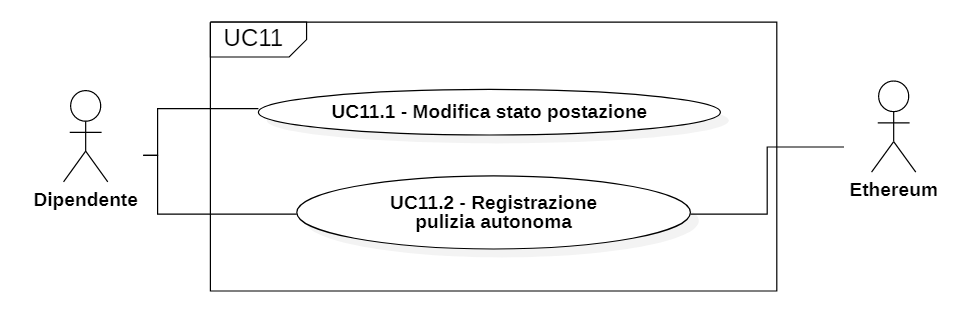
\includegraphics[width=15cm]{res/images/UC11.png}
	\caption{Segnalazione presenza}
	\label{fig:Segnalazione presenza}
\end{figure}
\begin{itemize}
	\item\textbf{Attori Primari:} dipendente.
	\item\textbf{Attori Secondari:} tag RFID, Ethereum.
	\item\textbf{Descrizione:} l’utente segnala in tempo reale la propria presenza alla postazione, appoggiando lo smartphone sul tag RFID. Inoltre, registra il tempo di inizio e di fine di questa azione grazie all'utilizzo di Ethereum.
	\item\textbf{Scenario principale:} l’utente appoggia lo smartphone sul tag RFID e segnala in questo modo la propria presenza.
	Il tempo di inizio e di fine di questa azione vengono memorizzati grazie all'utilizzo di Ethereum.
	\item\textbf{Precondizione:} l’utente si è autenticato nell'applicazione mobile e occupa una postazione.
	\item\textbf{Postcondizione:} l’utente segnala in tempo reale la presenza alla postazione e registra questa azione su Ethereum.
	\item\textbf{Estensioni:} 
	\begin{itemize}
		\item[$-$] visualizzazione errore: se l'utente sposta lo smartphone dal tag RFID (ad esempio per una telefonata), 
		dopo un timeout di qualche minuto, viene visualizzato un messaggio di errore (UC11.2);
		\item[$-$] visualizzazione errore: se l'utente si dimentica di premere il bottone di fine occupazione della postazione, viene visualizzato un messaggio di errore (UC11.4).
	\end{itemize}
\end{itemize}
\subsubsection{ UC11.1 - Presenza in tempo reale}
\begin{itemize}
	\item\textbf{Attori Primari:} dipendente.
	\item\textbf{Attori Secondari:} tag RFID.
	\item\textbf{Descrizione:} l’utente segnala in tempo reale la presenza alla postazione, appoggiando lo smartphone sul tag RFID.
	\item\textbf{Scenario principale:} l’utente appoggia lo smartphone sul tag RFID e segnala in questo modo la propria presenza in tempo reale.
	\item\textbf{Precondizione:} l’utente occupa una postazione e ha attivato nel proprio smartphone la possibilità di effettuare scansioni con tag RFID.
	\item\textbf{Postcondizione:} l’utente segnala in tempo reale la presenza alla postazione.
\end{itemize}
\subsubsection{ UC11.2 - Visualizzazione errore spostamento smartphone}
\begin{itemize}
	\item\textbf{Attori Primari:} dipendente.
	\item\textbf{Descrizione:} l’utente visualizza un messaggio di errore in quanto sposta lo smartphone dal tag RFID.
	\item\textbf{Scenario principale:} viene visualizzato un messaggio di errore che consiglia di riposizionare lo smartphone correttamente sul tag RFID.
	\item\textbf{Precondizione:} l’utente sposta il proprio smartphone dal tag RFID.
	\item\textbf{Postcondizione:} viene visualizzato un messaggio di errore specifico.
\end{itemize}
\subsubsection{ UC11.3 - Registrazione presenza}
\begin{itemize}
	\item\textbf{Attori Primari:} dipendente.
	\item\textbf{Attori Secondari:} Ethereum.
	\item\textbf{Descrizione:} l’utente registra l'inizio e la fine della propria occupazione della postazione.
	\item\textbf{Scenario principale:} l’utente sta navigando nella sezione della segnalazione della presenza e preme i bottoni di inizio e fine occupazione della postazione,
	nei corrispondenti momenti. Questa azione viene registrata grazie a Ethereum.
	\item\textbf{Precondizione:} l’utente occupa una postazione e preme i bottoni di inizio e fine dell'occupazione della postazione.
	\item\textbf{Postcondizione:} l'azione della precondizione viene registrata.
\end{itemize}
\subsubsection{ UC11.4 - Visualizzazione errore fine occupazione}
\begin{itemize}
	\item\textbf{Attori Primari:} dipendente.
	\item\textbf{Descrizione:} l’utente visualizza un messaggio di errore in quanto si dimentica di segnalare la fine dell'occupazione della postazione.
	\item\textbf{Scenario principale:} dopo un periodo di tempo abbastanza lungo, viene visualizzato un messaggio di errore in cui si notifica
	all'utente la fine della sua occupazione della postazione.
	\item\textbf{Precondizione:} l’utente non preme il bottone per la fine dell'occupazione della postazione.
	\item\textbf{Postcondizione:} viene visualizzato un messaggio di errore specifico.
\end{itemize}
\subsubsection{ UC12 - Pulizia autonoma}
\begin{figure}[H]
	\centering
	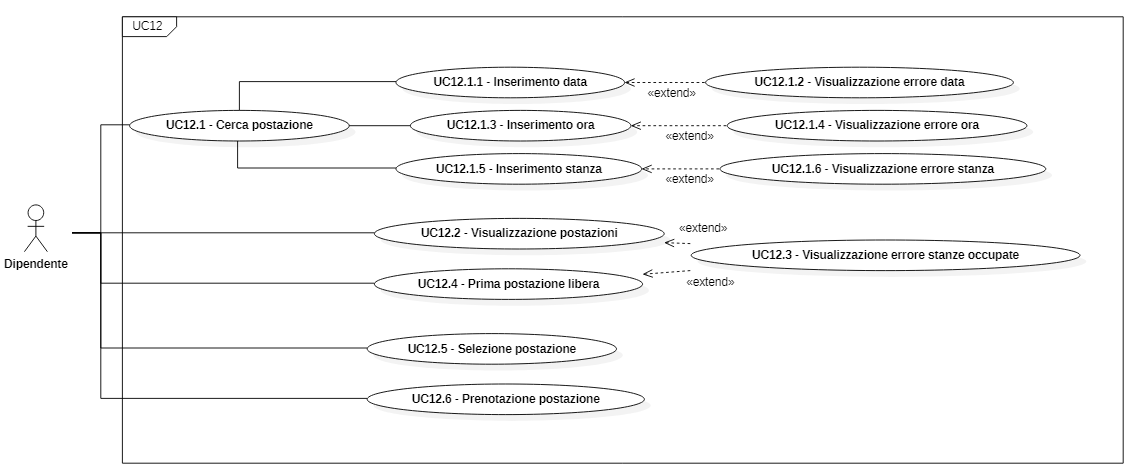
\includegraphics[width=15cm]{res/images/UC12.png}
	\caption{Pulizia autonoma}
	\label{fig:Pulizia autonoma}
\end{figure}
\begin{itemize}
	\item\textbf{Attori Primari:} dipendente.
	\item\textbf{Attori Secondari:} Ethereum.
	\item\textbf{Descrizione:} l’utente pulisce in autonomia la postazione e lo segnala sull'applicazione mobile. Inoltre, 
	registra di aver effettuato questa azione, grazie all'utilizzo di Ethereum.	\item\textbf{Scenario principale:} l’utente dopo aver igienizzato la postazione con il kit aziendale, modifica lo stato della postazione in libera e igienizzata. Inoltre, 
	registra di aver effettuato questa azione, grazie all'utilizzo di Ethereum.
	\item\textbf{Precondizione:} l’utente è autenticato nell'applicazione mobile, ha igienizzato la propria postazione e sta navigando nella sezione per la pulizia 
	autonoma della postazione.
	\item\textbf{Postcondizione:} l’utente modifica lo stato della postazione in libera e igienizzata e registra l'avvenuta pulizia autonoma della postazione.
\end{itemize}
\subsubsection{ UC12.1 - Modifica stato postazione }
\begin{itemize}
	\item\textbf{Attori Primari:} dipendente.
	\item\textbf{Descrizione:} l’utente dopo aver igienizzato autonomamente la postazione con il kit aziendale, modifica lo stato della stessa.
	\item\textbf{Scenario principale:} l’utente modifica lo stato della postazione in libera e igienizzata.
	\item\textbf{Precondizione:} l’utente sta navigando all'interno della sezione pulizia autonoma delle postazioni.
	\item\textbf{Postcondizione:} l’utente modifica lo stato della postazione.
\end{itemize}

\subsubsection{ UC12.2 - Registrazione pulizia autonoma }
\begin{itemize}
	\item\textbf{Attori Primari:} dipendente.
	\item\textbf{Attori Secondari:} Ethereum.
	\item\textbf{Descrizione:} l’utente segnala all'applicazione mobile di aver igienizzato autonomamente la postazione con il kit aziendale.
	\item\textbf{Scenario principale:} l’utente igienizza la postazione con il kit aziendale e registra questa azione grazie all'utilizzo di Ethereum.
	\item\textbf{Precondizione:} l’utente è autenticato nell'applicazione mobile, ha pulito la postazione e sta navigando nella sezione di 
	registrazione della pulizia autonoma.
	\item\textbf{Postcondizione:} l’utente registra l'avvenuta igienizzazione autonoma della postazione.
\end{itemize}
\subsubsection{ UC13 - Gestione prenotazione }
\begin{figure}[H]
	\centering
	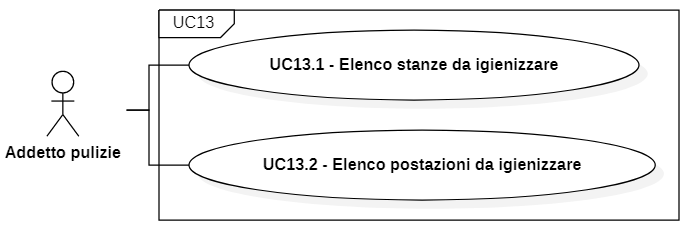
\includegraphics[width=18cm]{res/images/UC13.png}
	\caption{Gestione prenotazione}
	\label{fig:Gestione prenotazione}
\end{figure}
\begin{itemize}
	\item\textbf{Attori Primari:} dipendente.
	\item\textbf{Descrizione:} l’utente vuole prenotare una postazione di una stanza in un determinato giorno e orario.
	\item\textbf{Scenario principale:} l’utente ha visualizzato o gestito le prenotazioni di una stanza all’interno del sistema.
	\item\textbf{Precondizione:} l’utente si è autenticato nell'applicazione mobile e sta navigando nella sezione di gestione delle prenotazioni.
	\item\textbf{Postcondizione:} l’utente ha visualizzato o gestito le prenotazioni all’interno del sistema.
\end{itemize}
\subsubsection{ UC13.1 - Cerca postazione}
\begin{itemize}
	\item\textbf{Attori Primari:} dipendente.
	\item\textbf{Descrizione:} l’utente vuole prenotare una postazione di una stanza in un determinato giorno e orario.
	\item\textbf{Scenario principale:} 
	\begin{itemize}
		\item[$-$] l’utente inserisce la data (UC13.1.1);
		\item[$-$] l’utente inserisce l'orario (UC13.1.3);
		\item[$-$] l’utente inserisce l'identificativo della stanza (UC13.1.5).
	\end{itemize}
	\item\textbf{Precondizione:} l’utente sta navigando nella sezione dell'applicazione dedicata alla ricerca di una postazione.
	\item\textbf{Postcondizione:} l’utente inserisce i campi necessari alla ricerca della postazione desiderata.
\end{itemize}
\subsubsection{ UC13.1.1 - Inserimento data }
\begin{itemize}
	\item\textbf{Attori Primari:} dipendente.
	\item\textbf{Descrizione:} l’utente sta cercando una postazione disponibile e deve compilare il campo della data.
	\item\textbf{Scenario principale:} l’utente ha compilato il campo data.
	\item\textbf{Precondizione:} l’utente sta compilando i campi richiesti per effettuare la ricerca.
	\item\textbf{Postcondizione:} l’utente ha compilato il campo richiesto.
	\item\textbf{Estensioni:} l’utente inserisce i campi necessari alla ricerca della postazione desiderata.
	\begin{itemize}
		\item[$-$] l’utente inserisce una data non valida (UC13.1.2);
	\end{itemize}
\end{itemize}
\subsubsection{ UC13.1.2 - Visualizzazione errore: data non valida  }
\begin{itemize}
	\item\textbf{Attori Primari:} dipendente.
	\item\textbf{Descrizione:} l’utente ha compilato un campo per la data, ma è in un formato non corretto.
	\item\textbf{Scenario principale:} 
	\begin{itemize}
		\item[$-$] l’utente ha inserito il campo per la data;
		\item[$-$] il sistema elabora la richiesta;
		\item[$-$] viene visualizzato un errore che segnala che la data non è valida.
	\end{itemize}
	\item\textbf{Precondizione:} l’utente ha compilato il campo per la data.
	\item\textbf{Postcondizione:} l’utente visualizza un messaggio di errore specifico e non porta a termine l’azione.
	\item\textbf{Estensioni:} l’utente inserisce i campi necessari alla ricerca della postazione desiderata.
	\begin{itemize}
		\item[$-$] l’utente inserisce un orario non valido (UC13.1.4);
	\end{itemize}
\end{itemize}
\subsubsection{ UC13.1.3 - Inserimento ora }
\begin{itemize}
	\item\textbf{Attori Primari:} dipendente.
	\item\textbf{Descrizione:} l’utente sta cercando una postazione disponibile e deve compilare il campo orario con granularità di un'ora.
	\item\textbf{Scenario principale:} l’utente ha compilato il campo orario.
	\item\textbf{Precondizione:} l’utente sta compilando i campi richiesti per effettuare la ricerca.
	\item\textbf{Postcondizione:} l’utente ha compilato il campo richiesto.
	\item\textbf{Estensioni:} l’utente inserisce i campi necessari alla ricerca della postazione desiderata.
	\begin{itemize}
		\item[$-$] l’utente inserisce una stanza non valida (UC13.1.6).
	\end{itemize}
\end{itemize}
\subsubsection{ UC13.1.4 - Visualizzazione errore: orario non valido }
\begin{itemize}
	\item\textbf{Attori Primari:} dipendente.
	\item\textbf{Descrizione:} l’utente ha compilato un campo per l'orario, ma è in un formato non corretto.
	\item\textbf{Scenario principale:} 
	\begin{itemize}
		\item[$-$] l’utente ha inserito il campo per l'orario;
		\item[$-$] il sistema elabora la richiesta;
		\item[$-$] viene visualizzato un errore che segnala che l'orario non è valido.
	\end{itemize}
	\item\textbf{Precondizione:} l’utente ha compilato il campo per l'orario.
	\item\textbf{Postcondizione:} l’utente visualizza un messaggio di errore specifico e non porta a termine l’azione.
\end{itemize}
\subsubsection{ UC13.1.5 - Inserimento stanza }
\begin{itemize}
	\item\textbf{Attori Primari:} dipendente.
	\item\textbf{Descrizione:} l’utente sta cercando una postazione disponibile e deve compilare il campo dell'identificativo della stanza.
	\item\textbf{Scenario principale:} l’utente ha compilato il campo dell'identificativo della stanza.
	\item\textbf{Precondizione:} l’utente sta compilando i campi richiesti per effettuare la ricerca.
	\item\textbf{Postcondizione:} l’utente ha compilato il campo richiesto.
\end{itemize}
\subsubsection{ UC13.1.6 - Visualizzazione errore: stanza non valida }
\begin{itemize}
	\item\textbf{Attori Primari:} dipendente.
	\item\textbf{Descrizione:} l’utente ha compilato un campo per l'identificativo della stanza, ma è in un formato non corretto.
	\item\textbf{Scenario principale:} 
	\begin{itemize}
		\item[$-$] l’utente ha inserito il campo per l'identificativo della stanza;
		\item[$-$] il sistema elabora la richiesta;
		\item[$-$] viene visualizzato un errore che segnala che l'identificativo della stanza non è valido.
	\end{itemize}
	\item\textbf{Precondizione:} l’utente ha compilato il campo per la stanza.
	\item\textbf{Postcondizione:} l’utente visualizza un messaggio di errore specifico e non porta a termine l’azione.
\end{itemize}
\subsubsection{ UC13.2 - Visualizzazione postazioni  }
\begin{itemize}
	\item\textbf{Attori Primari:} dipendente.
	\item\textbf{Descrizione:} l’utente visualizza le postazioni con colori diversi in base allo stato. L'identificativo di una postazione è costituito da una lettera seguita da un numero (ad esempio: D10). 
	\item\textbf{Scenario principale:} viene visualizzato lo schema delle postazioni, rappresentato con colori diversi in base allo stato in cui si trovano.
	\item\textbf{Precondizione:} l’utente ha inserito i campi data, orario e stanza correttamente e premuto il bottone di ricerca, nella sezione 
	medesima.
	\item\textbf{Postcondizione:} l’utente visualizza le postazioni nella stanza.
	\item\textbf{Estensioni:}
	\begin{itemize}
		\item[$-$] visualizzazione errore: tutte le postazioni nella stanza selezionata sono occupate o guaste (UC13.3).
	\end{itemize}
\end{itemize}
\subsubsection{ UC13.3 - Visualizzazione errore: postazioni occupate }
\begin{itemize}
	\item\textbf{Attori Primari:} dipendente.
	\item\textbf{Descrizione:} l’utente visualizza un messaggio di errore, in quanto non ci sono postazioni prenotabili.
	\item\textbf{Scenario principale:} 
	\begin{itemize}
		\item[$-$] l’utente ha inserito i campi data, orario, stanza;
		\item[$-$] il sistema elabora la richiesta;
		\item[$-$] viene visualizzato un messaggio di errore che consiglia di selezionare un'altra fascia oraria o stanza.
	\end{itemize}
	\item\textbf{Precondizione:} l’utente ha compilato i campi data, orario, stanza oppure ha selezionato la sezione prima postazione 
	disponibile (UC13.4).
	\item\textbf{Postcondizione:} l’utente visualizza un messaggio di errore specifico e non porta a termine l’azione.
\end{itemize}
\subsubsection{ UC13.4 - Prima postazione libera }
\begin{itemize}
	\item\textbf{Attori Primari:} dipendente.
	\item\textbf{Descrizione:} l’utente riceve l'identificativo di una postazione igienizzata e libera in una determinata stanza, 
	in modo automatico e in base a un criterio di distanziamento dalle altre postazioni.
	\item\textbf{Scenario principale:} viene fornito l'identificativo di una postazione libera e igienizzata, oppure di una libera e non igienizzata (si veda UC10).
	\item\textbf{Precondizione:} l’utente preme il bottone nella sezione della prima postazione disponibile.
	\item\textbf{Postcondizione:} l’utente riceve l'identificativo di una postazione.
	\item\textbf{Estensioni:}
	\begin{itemize}
		\item[$-$] tutte le postazioni nella stanza selezionata sono occupate o guaste (UC13.3).
	\end{itemize}
\end{itemize}
\subsubsection{ UC13.5 - Selezione postazione }
\begin{itemize}
	\item\textbf{Attori Primari:} dipendente.
	\item\textbf{Descrizione:} l’utente dopo aver visualizzato le postazioni con colori diversi in base allo stato, ne seleziona una. E' possibile scegliere una postazione libera e igienizzata o non igienizzata.
	\item\textbf{Scenario principale:} viene selezionata una postazione.
	\item\textbf{Precondizione:} l’utente ha visualizzato correttamente le postazioni di una stanza.
	\item\textbf{Postcondizione:} l’utente seleziona una postazione.
\end{itemize}
\subsubsection{ UC13.6 - Prenotazione postazione }
\begin{itemize}
	\item\textbf{Attori Primari:} dipendente.
	\item\textbf{Descrizione:} l’utente dopo aver selezionato la postazione, effettua la prenotazione. 
	\item\textbf{Scenario principale:} l’utente sta navigando nella sezione per la prenotazione di una postazione
	e preme il bottone per effettuare questa azione.
	\item\textbf{Precondizione:} l’utente ha selezionato correttamente la postazione di una stanza.
	\item\textbf{Postcondizione:} l'utente prenota la postazione.
	\item\textbf{Estensioni:}
	\begin{itemize}
		\item[$-$] nel caso in cui l'utente scelga di prenotare una postazione libera e sporca si veda UC12,
		per poi tornare allo scenario principale (13.7).
	\end{itemize}
\end{itemize}
\subsubsection{ UC14 - Elenco stanze e postazioni da igienizzare}
\begin{figure}[H]
		\centering
		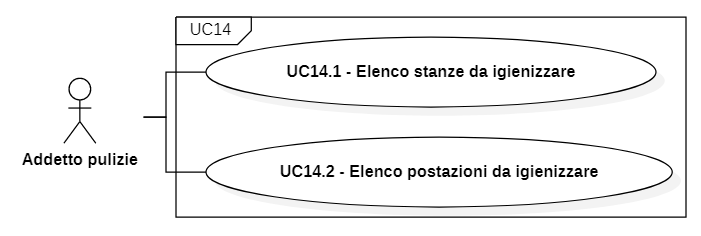
\includegraphics[width=15cm]{res/images/UC14.png}
		\caption{Elenco stanze e postazioni da igienizzare}
		\label{fig:Elenco stanze e postazioni da igienizzare}
	\end{figure}
\begin{itemize}
           	\item\textbf{Attori Primari:} addetto pulizie.
           	\item\textbf{Descrizione:} l'utente riceve un elenco delle postazioni(UC14.2) e delle stanze(UC14.1) che necessitano di igienizzazione.
           	\item\textbf{Scenario principale:} l'utente si trova all'interno del sistema e verifica tutte le postazioni che sono state utilizzate almeno da un dipendente, che saranno quindi da igienizzare, oppure può decidere di igienizzare l’intera stanza.
           	\item\textbf{Precondizione:} l'utente va nella sezione dedicata nel sistema e deve premere un bottone.
           	\item\textbf{Postcondizione:} l'utente verifica quali postazioni sono state occupate da almeno un dipendente, così da ottenere un elenco delle stanze e postazioni da igienizzare.
\end{itemize}

\subsubsection{UC14.1 - Elenco stanze da igienizzare}
\begin{itemize}
           	\item\textbf{Attori Primari:} addetto pulizie.
           	\item\textbf{Descrizione:} l'utente riceve un elenco delle stanze che necessitano di igienizzazione.
           	\item\textbf{Scenario principale:} l'utente si trova all'interno del sistema e verifica tutte le stanze che sono state utilizzate almeno da un dipendente, che saranno quindi da igienizzare.
           	\item\textbf{Precondizione:} l'utente va nella sezione dedicata nel sistema e deve premere un bottone.
           	\item\textbf{Postcondizione:} l'utente verifica quali stanze sono state occupate da almeno un dipendente, così da ottenere un elenco delle stanze da igienizzare.
\end{itemize}
\subsubsection{UC14.2 - Elenco postazioni da igienizzare}
\begin{itemize}
           	\item\textbf{Attori Primari:} addetto pulizie.
           	\item\textbf{Descrizione:} l'utente riceve un elenco delle postazioni che necessitano di igienizzazione.
           	\item\textbf{Scenario principale:} l'utente si trova all'interno del sistema e verifica tutte le postazioni che sono state utilizzate almeno da un dipendente, che saranno quindi da igienizzare.
           	\item\textbf{Precondizione:} l'utente va nella sezione dedicata nel sistema e deve premere un bottone.
           	\item\textbf{Postcondizione:} l'utente verifica quali postazioni sono state occupate da almeno un dipendente, così da ottenere un elenco delle postazioni da igienizzare.
\end{itemize}

\subsubsection{ UC15 - Marcatura stanza e postazione come igienizzata}
\begin{figure}[H]
		\centering
		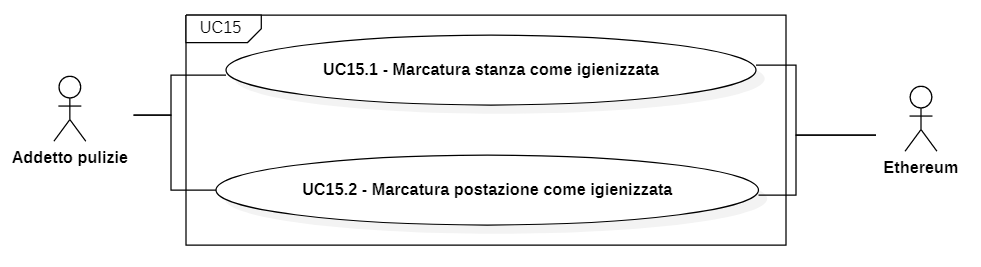
\includegraphics[width=18cm]{res/images/UC15.png}
		\caption{Marcatura stanza e postazione come igienizzata}
		\label{fig:Marcatura stanza e postazione come igienizzata}
	\end{figure}
\begin{itemize}
           	\item\textbf{Attori Primari:} addetto pulizie.
		\item\textbf{Attori Secondario:} Ethereum.
           	\item\textbf{Descrizione:} dopo l'igienizzazione l'utente marca le stanze o le postazioni che ha pulito come igienizzate.
           	\item\textbf{Scenario principale:} l'utente igienizza la stanza(UC15.1) o la postazione(UC15.2), in seguito accede al sistema e la marca come igienizzata attraverso l'utilizzo di Ethereum.
           	\item\textbf{Precondizione:} l'utente ottiene l'elenco delle stanze e delle postazioni da igienizzare.
           	\item\textbf{Postcondizione:} l'utente, dopo l'igienizzazione, marca le stanze e le postazioni come igienizzate.
\end{itemize}
\subsubsection{UC15.1 - Marcatura stanza come igienizzata}
\begin{itemize}
           	\item\textbf{Attori Primari:} addetto pulizie.
		\item\textbf{Attori Secondario:} Ethereum.
           	\item\textbf{Descrizione:} dopo l'igienizzazione l'utente marca la stanza come igienizzata.
           	\item\textbf{Scenario principale:} l'utente igienizza la stanza, in seguito accede al sistema e la marca come igienizzata attraverso l'utilizzo di Ethereum.
           	\item\textbf{Precondizione:} l'utente ottiene l'elenco delle stanze da igienizzare.
           	\item\textbf{Postcondizione:} l'utente, dopo l'igienizzazione, marca le stanze come igienizzate.
\end{itemize}
\subsubsection{UC15.2 - Marcatura postazione come igienizzata}
\begin{itemize}
           	\item\textbf{Attori Primari:} addetto pulizie.
		\item\textbf{Attori Secondario:} Ethereum.
           	\item\textbf{Descrizione:} dopo l'igienizzazione l'utente marca la postazione come igienizzata.
           	\item\textbf{Scenario principale:} l'utente igienizza la postazione, in seguito accede al sistema e la marca come igienizzata attraverso l'utilizzo di Ethereum.
           	\item\textbf{Precondizione:} l'utente ottiene l'elenco delle postazioni da igienizzare.
           	\item\textbf{Postcondizione:} l'utente, dopo l'igienizzazione, marca le postazioni come igienizzate.
\end{itemize}
